\scanpage{9}
\mspage{2}
i.e. on a, pour \(\deleted{x}\xi\in J_n(n')\) i.e. \(x\in J_n,\ \tau_n(x)=n'\)
\[
 u_\xi(d_{n'})=\xi .
\]
\deleted{De} \unsure{plus,|\deleted{plus,}} \unsure{fort|faut|fut} encore,
% The brace beneath ``on a :'' has a long right end rising above the line.
\(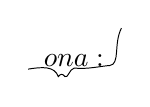
\begin{tikzpicture}[baseline=(ona.base),x=1em,y=1em]
 \node[inner sep=0pt] (ona) at (0,0) {$\text{on a :}$};
 \draw[line width=.35pt] (-1.65,-.30)
  .. controls (-1.15,-.22) and (-.70,-.18) .. (-.56,-.57)
  .. controls (-.49,-.48) and (-.42,-.44) .. (-.32,-.57)
  .. controls (-.20,-.64) and (-.17,-.30) .. (.02,-.26)
  .. controls (.45,-.32) and (1.05,-.18) .. (1.30,-.17)
  .. controls (1.68,-.12) and (1.43,.62) .. (1.72,1.18);
\end{tikzpicture}\)
\inserted{\(u_\xi\) induit un isom} \(J_{n'}\xrightarrow{\overset{u_\xi}{\sim}}(J_n)_{\leq\xi}\)

Lorsque \(n'=n\), on a \(J_{n,n}=\{d_n\}\), et
\[
 u_{d_n}=\mathrm{id}_{J_n}
\]

La connaissance de \(\mathbb N,\ (J_n)_{n\in\mathbb N},\ (\tau_n)_{n\in\mathbb N},\
(\rho_{n,n'})_{\substack{(n',\deleted{\unsure{n'|m}}n)\in\mathbb N\times\mathbb N\\ n'\leq n}}\) permet de reconstituer \deleted{à peu de \unsure{chose|choses} près} \deleted{essentiellement \unsure{la|le} sous-catégorie pleine}\inserted{la catégorie} \(M\), à \deleted{il} équiv \unsure{prés|près}, il manque encore une \deleted{\unsure{description|descripteur}} \inserted{condition} pour composer les hom ``standart entre les \(J_n\), i.e ceux provenant des \(J_{n',n'}\). \deleted{Donc} On considère une situation
\diagram{\begin{tikzcd}[ampersand replacement=\&,column sep=.8em,row sep=small]
 \& \& \eta \&[1.2em] \& \xi\\[-.8em]
 \& \& \rotatebox{-90}{\(\in\)} \& \& \rotatebox{-90}{\(\in\)}\\
 J_{n''}\arrow[rr,"{u^{n'}_{\eta}}"{pos=.32,inner sep=0pt}] \& \& J_{n'}\arrow[rr,"{u_\xi^n}"{pos=.27,inner sep=0pt,yshift=-.3em}] \& \& J_n\\[.5em]
 n'' \& \leq \& n' \& \leq \& n
\end{tikzcd}}
% Both turned membership arches open downward. The second xi descender crosses
% its arrow shaft; labels lie toward the left portions of unequal arrow spans.
on doit avoir
\[
 u_\xi^n\,u_\eta^{n'}=u_{\deleted{\unsure{a|\xi}}\zeta}^{n}
 \qquad\text{où}\quad \zeta=u_\xi^n(\eta)
 % A separate small point lies above-right of this equals sign; no role assigned.
 \mathrel{\begin{tikzpicture}[baseline=(eq.base),x=1em,y=1em]
  \node[inner sep=0pt] (eq) at (0,0) {$=$};
  \fill (.20,.52) circle (.30pt);
 \end{tikzpicture}}
 (u_\xi^n\,u_\eta^{n'})(d_{n''})
\]
qui exprime la \deleted{\unsure{composition|stabilité|compatibilité|stabilis}} stabilité de la notion d'hom admissible entre. \(J_n\) par composition.

\deleted{Il est évident que la \unsure{catég|caté}} \inserted{Soit \(M_0\) la catégorie définie par}
\[
 \mathrm{Ob}\,M_0=\mathbb N,\quad \mathrm{Hom}_{M_0}(n',n)=
 \left\{\begin{aligned}
 &\varnothing\ \text{si }n'\nleq n\\
 &\text{ens. des hom. admissibles}\\
 &\qquad J_{n'}\to J_n\quad\text{si }n'\leq n
 \end{aligned}\right.
\]
% archive sheet number: 8
